\documentclass[12pt]{article}
\usepackage[utf8]{inputenc}
\usepackage[a4paper, width=150mm, top=25mm, bottom=25mm]{geometry}

\usepackage{titlesec}
\newcommand{\sectionbreak}{\clearpage}

\usepackage{natbib}
\usepackage{graphicx}
\usepackage{imakeidx}
\usepackage{caption}
\usepackage{listings}
%\usepackage[parfill]{parskip}  lineas entre párrafos

\usepackage{hyperref}
\hypersetup{
    colorlinks=true,
    linkcolor=blue,
    filecolor=magenta,      
    urlcolor=cyan,
}

%%%%%%%%%%%%%%%%%%%%%%%%%%%
%%        EDICION        %%
%%%%%%%%%%%%%%%%%%%%%%%%%%%

\usepackage{todonotes}

%%%%%%%%%%%%%%%%%%%%%%%%%%%
\renewcommand{\lstlistingname}{Archivo}
%%%%%%%%%%%%%%%%%%%%%%%%%%%

\graphicspath{ {images/} }
\makeindex


% Title data
\title{Control parental de accesos WiFi}
\author{Esteban Omelio Puentes Silveira}
\date{Mayo, 2017}

\begin{document}
\maketitle

%\begin{figure}[h!]
%    \centering
%        \includegraphics[scale=0.2]{logo_uvigo.png}
%        \caption*{Universidad de Vigo}
%        \label{fig:uvigo}
%\end{figure}

\clearpage

%%%%%%%%%%%%%%%%%%%%%%%%%%%%%%%%%%%
%% DEDICATORIA Y AGRADECIMIENTOS
%%%%%%%%%%%%%%%%%%%%%%%%%%%%%%%%%%%

\section{Dedicatoria}
A Patry, el amor de mi vida

\section{Agradecimientos}
A mi cuñado Daniel Victor por apoyarme durante todo este tiempo en la univerisdad


%%%%%%%%%%%%%%%%%%%%%%%%%%%%%%%%%%%
%% ÍNDICE
%%%%%%%%%%%%%%%%%%%%%%%%%%%%%%%%%%%

\renewcommand\contentsname{Índice}
\tableofcontents
\printindex


%%%%%%%%%%%%%%%%%%%%%%%%%%%%%%%%%%%
%% CONTENIDO
%%%%%%%%%%%%%%%%%%%%%%%%%%%%%%%%%%%
\todo{márgenes iniciales de las secciones}
\todo{espacio entre párrafos}
\todo{saltos de líneas en enumereates e itemizes}
\todo{hojas impares (openright https://tex.stackexchange.com/questions/36988/regarding-the-book-report-and-article-document-classes-what-are-the-mai)}
\section{Introducción}
%haberá que incluír unha introdución ao problema e xustificación do
%traballo realizado. En caso de que o TFG integre ou desenvolva traballos feitos na
%actividade doutras materias da titulación, o/a estudante deberá especificar os devanditos
%traballos e materias nesta sección.*/

Internet, desde su creación, ha sido un medio cada vez más accesible; actualmente cuenta con 3,731,973,423 de usuarios, cifra que representa casi el 50\% de los habitantes del planeta. 

El uso de redes Wi-Fi ha permitido que los usuarios tengan una mayor disponibilidad de la conexión a Internet llevándola a sus dispositivos móviles, tanto en casa como fuera de ella. Actualmente es común que los menores de edad dispongan de dispositivos móviles desde los cuales puedan acceder a Internet, sin embargo, esto conlleva a que debido a su inmadurez y falta de experiencia, terminen pasando más tiempo del recomendado frente a una pantalla, sin dedicarle el tiempo necesario a sus obligaciones, desatendiendo sus estudios o directamente perdiendo la comunicación con los seres que lo rodean. Los padres de los menores normalmente toman medidas para prevenir 



\section{Objetivos}
% presentar o problema que se vai tratar, incluír o obxectivo principal e os
% específicos, de ser o caso, do traballo presentado, indicando o alcance para cada un deles.
    Realizar un estudio de necesidades generales teniendo en cuenta las características de los routers domésticos y con los resultados obtenidos crear un sistema capaz de controlar redes Wi-Fi similares a las que comunmente pueden ser encontradas en los hogares, de forma que los padres y madres puedan limitar el uso de Internet a los menores y las menores de forma sencilla y sin necesitar conocimientos avanzados de informática.

    \begin{enumerate}
        \item El sistema debe poder ser controlado desde un dispositivo móvil:
        \begin{itemize}
            \item Conectado a la red Wi-Fi del propio router.
            \item Conectado a Internet y accediendo desde la interfaz WAN.\todo{referenciar}
        \end{itemize}

        \item Incluir control para encender y apagar la red Wi-Fi de forma sencilla.
        \item Implementar la gestión de un filtro MAC \todo{referenciar}, este debe contar con diferentes estados:
            \begin{itemize}
                \item \textbf{Desactivado:} Permite que todos los dispositivos puedan tener acceso a la red Wi-Fi.
                \item \textbf{Permitir:} Solamente permite que sean conectados a la red Wi-Fi los dispositivos explícitamente especificados. 
                \item \textbf{Denegar:} Permite el acceso a la red Wi-Fi a todos los dispositivos excepto a los que sean explícitamente especificados.
            \end{itemize}
        \item Aplicar un mecanismo de seguridad que elimine la posibilidad de que se pueda tomar el control del router desde un dispositivo móvil no autorizado.
        \item Aplicar un mecanismo de seguridad capaz de impedir la réplica de paquetes de red que permitan cambiar configuraciones een el router de forma desautorizada.
        \item Añadir soporte para idiomas
    \end{enumerate}


\section{Resumen de la solución propuesta}
% indicarase a solución aportada para o problema
% presentado. Deberase incluír aquí a metodoloxía empregada.
    Tras realizar un análisis de los componentes con los que comunmente se cuenta en entornos domésticos, se ha concluido que no es posible crear una solución estándar para los diferentes proveedores de servicios de Internet, por tanto, se plantea la realización de un sistema de control parental sobre accesos Wi-Fi en un router con OpenWRT, un sistema operativo compatible con un gran número de los routers actuales del mercado y adaptable a la mayoría de los existentes. Se creará una App sobre Android para el control de los dispositivos conectados a la red Wi-Fi doméstica, y una aplicación que se ejecute como demonio en el router, donde se recibirán conexiones desde la App con la configuración a establecer. La conexión se realizará mediante paquetes UDP, evitando así el establecimiento de conexión y ganando en velociadad.

    La funcionalidades de la aplicación se desarrollarán utilizando los propios mecanismos proporcionados por OpenWRT para el control de sus sistemas. El apagado/encendido de la red Wi-Fi se realizará a través del comando \textit{wifi} con los argumentos necesarios en cada caso, mientras que la gestión del control de accesos se llevará a cabo mediante los archivos de configuración de unicados en \textit{/etc/config}.

    Para llevar a cabo la creación de este sistema, inicialmente se valoró el uso de una metodología de desarrollo en cascada, sin embargo, tras una nueva aproximación al problema, se ha llegado a la conclusión de que esta no era la solución más acertada debido a que el sistema se basa en un entorno de red, además se necesita realizar compilación cruzada utilizando un SDK específico, el cual cuenta con sus propias librerías, y la documentación de la que se dispone puede estar incompleta, desactualizada o errónea en su totalidad. Esto lleva como consecuencia que se necesite realizar pruebas de envíos de paquetes constantemente, y que debido a la diferencia de librerías se requiera realizar cambios en el código que se plantee inicialmente. También es necesario que el sistema ocupe el menor espacio posible, ya que el espacio de almacenamiento en routers suele ser limitado, lo que llevará a que el codigo deba ser refactorizado constantemente.
    
    Tras el análisis anterior se ha concluído que lo más adecuado sería el uso de un método ágil de desarrollo, en concreto \textit{Scrum}, que está más enfocado en la administración del desarrollo iterativo. \textit{Scrum} consta de 3 fases:
    
    \begin{itemize}
        \item Planificación de un \textit{boceto} donde se establecen los objetivos generales del proyecto y el diseño de la arquitectura del software.
        \item Una serie de ciclos \textit{sprint} donde cada ciclo desarrolla un incremento del sistema.
        \item \textit{Cierre} del proyecto donde se completa la documentación requerida como ayudas y manuales de usuario.
    \end{itemize}

    \textit{Scrum} permite que el producto se desglose en piezas comprensibles de forma individual y que son desarrolladas de forma iterativa, recibiendo retroalimentación del usuario con cada entrega y realizando cambios en consecuencia. Para llevar a cabo el desarrollo utilizando este método, es necesario ocupar los roles imprescindibles para su funcionamiento.

    \begin{itemize}
        \item \textbf{Equipo de desarrollo:} Equipo responsable de llevar a cabo el desarrollo del sistema. Este rol estará compuesto únicamente por el alumno.
        \item \textbf{Cliente:} Encargado de defininir los requisitos, utilizar las versiones resultantes de cada \textit{sprint} y aportar retroalimentación para la mejora del sistema. Este rol será llevado a cabo por el tutor del TFG.
        \item \textbf{Maestro de Scrum:} Encargado de restrar el trabajo que queda por hacer, tomar desiciones, medir el avance en función de la planificación inicial y mantener la comunicación con el cliente. Este rol será adoptado por el alumno.
    \end{itemize}

\section{Planificación y seguimiento}
% deberase incluír un diagrama de Gantt que amose tanto
% a planificación do traballo, coa súa distribución de fases e tarefas, e a súa comparación cos
% datos reais obtidos tras o desenvolvemento do traballo.

\section{Arquitectura y tecnologías}
% explicarase a arquitectura empregada para alcanzar os obxectivos propostos.

    \subsection{Arquitectura del sistema}

    \subsection{Tecnologías e integración de productos de terceros}
    % describiranse adecuadamente as tecnoloxías utilizadas para o desenvolvemento do traballo, así coma os diversos productos que non son da autoría do/da estudante, xustificando a súa utilización.

\section{Especificación y análisis de requisitos}
% describiranse os requisitos necesarios, tanto funcionais como non funcionais. Incluiranse os aspectos máis relevantes correspondentes á análise do traballo realizado.

\section{Diseño de software}
% (estático e dinámico) ou do hardware: indicaranse os aspectos máis relevantes correspondentes ao deseño do traballo realizado
% estatico -> diagrama de clases
% dinamico -> diagrama de secuencia, 

\section{Gestión de datos e información}
% Xestión de datos e información: describiranse os métodos ou técnicas empregadas para xestionar tanto os datos coma o resto de información relevante.
    Ya que el objetivo es crear un mecanismo de control para accesos a la red Wi-Fi, el sistema que se plantea no cuenta con bases de datos para almacenar información, sin embargo, se necesita una forma de guardar las configuraciones utilizadas.
    
    \subsection{Servidor}
        En el dispositivo servidor, para hacer uso de los mecanismos que brinda OpenWRT para la gestión de sus funcionalidades, se cuenta con un conjunto de archivos de configuración ubicados en la carpeta \textit{/etc/config}. En especial se hace uso del fichero \textit{wireless}, donde se almacenan las configuraciones hardware y software que son utilizadas para el funcionamiento la red Wi-Fi. \todo{referenciar archivo} A continuación se muestra un ejemplo de este.
        \todo{mirar si hay un paquete para bash}
        \todo{modificar comillas}
        \todo{modificar titulo: Eliminar listing 1}
        \todo{márgenes superiores e inferiores de textos y fotos}
        \begin{lstlisting}[caption=/etc/config/wireless, language=bash]
            config wifi-device `radio0'
                    option type `mac80211'
                    option hwmode `11g'
                    option path `pci0000:00/0000:00:01.0/ssb0:0'
                    option disabled `0'
                    option channel `4'
                    option txpower `20'
                    option country `00'

            config wifi-iface
                    option network `wwan'
                    option encryption `psk2'
                    option device `radio0'
                    option ssid `TFG_AccessPoint'
                    option mode `ap'
                    option key `wifitesting'

                    option macfilter `deny'
                    list maclist `B1:EE:A1:04:23:4E'
                    list maclist `B4:5D:83:4A:1B:50'
                    list maclist `0E:00:C1:FA:4E:98'
        \end{lstlisting}

        El parámetro \textit{wifi-device} indica la configuración de un dispositivo físico conectado al sistema, y al cual se le aplican las opciones que se definen debajo. En estas opciones se especifican parámetros como el tipo de dispositivo, la potencia y el canal que utilizará.

        El parámetro \textit{wifi-iface} indica la configuración de una interfaz inalámbrica, especificando en las opciones el dispositivo físico y la red OpenWRT (ya definidos) a la que estará vinculada. Además, también se definen opciones como el mecanismo de seguridad y el modo de operación del controlador de red. El sistema que se desarrolla, hace uso de las funciones que se encuentran al final del ejemplo.
        
        \begin{itemize}
            \item \textbf{mactiflter}: Indica la configuración a adoptar por el filtro MAC, esta se especifica entre comillas simples, y puede ser \textit{deny} o \textit{allow}. Para indicar que el filtro debe está desactivado se elimina toda la línea.
            \item \textbf{list maclist}: Es utilizada para especificar las direcciones MAC a las que se les va a aplicar el filtro, se pueden definir tantas opciones \textit{list maclist} como sea necesario.
        \end{itemize}

    \subsection{Cliente}
        En el dispositivo cliente, las configuraciones que se almacenan son las relacionadas a la conexión: \textit{Dirección IP}, \textit{Puerto} y \textit{Contraseña}, así como los \textit{Dispositivos} añadidos a la aplicación para gestionar el filtro MAC. También son almacenados los \textit{Estados} de los elementos de la interfaz de usuario que son utilizados para controlar el sistema.

        Para gestionar estos datos se utiliza \textit{SharedPreferences}, una forma de almacenamiento \textit{Clave-Valor} ofrecida por Android. Un objeto de este tipo tiene asociado un archivo donde se almacenan y proporciona métodos simples para leer y escribir dichos pares.
        
        Los procesos de lectura y escritura se realizan dentro de \textit{onResume()} y \textit{onPause()} respectivamente. El primero es ejecutado cuando la actividad es creada, iniciada o reanudada, mientras que el segundo es ejecutado cuando la actividad por cualquier motivo quede suspendida, la aplicación sea detenida o el proceso destruido. La imagen \ref{fig:androidlifecycle} muestra el orden de ejecución de los métodos en una actividad Android.
        
        \todo{que esto no quede solo}
        \begin{figure}[h!]
            \centering
                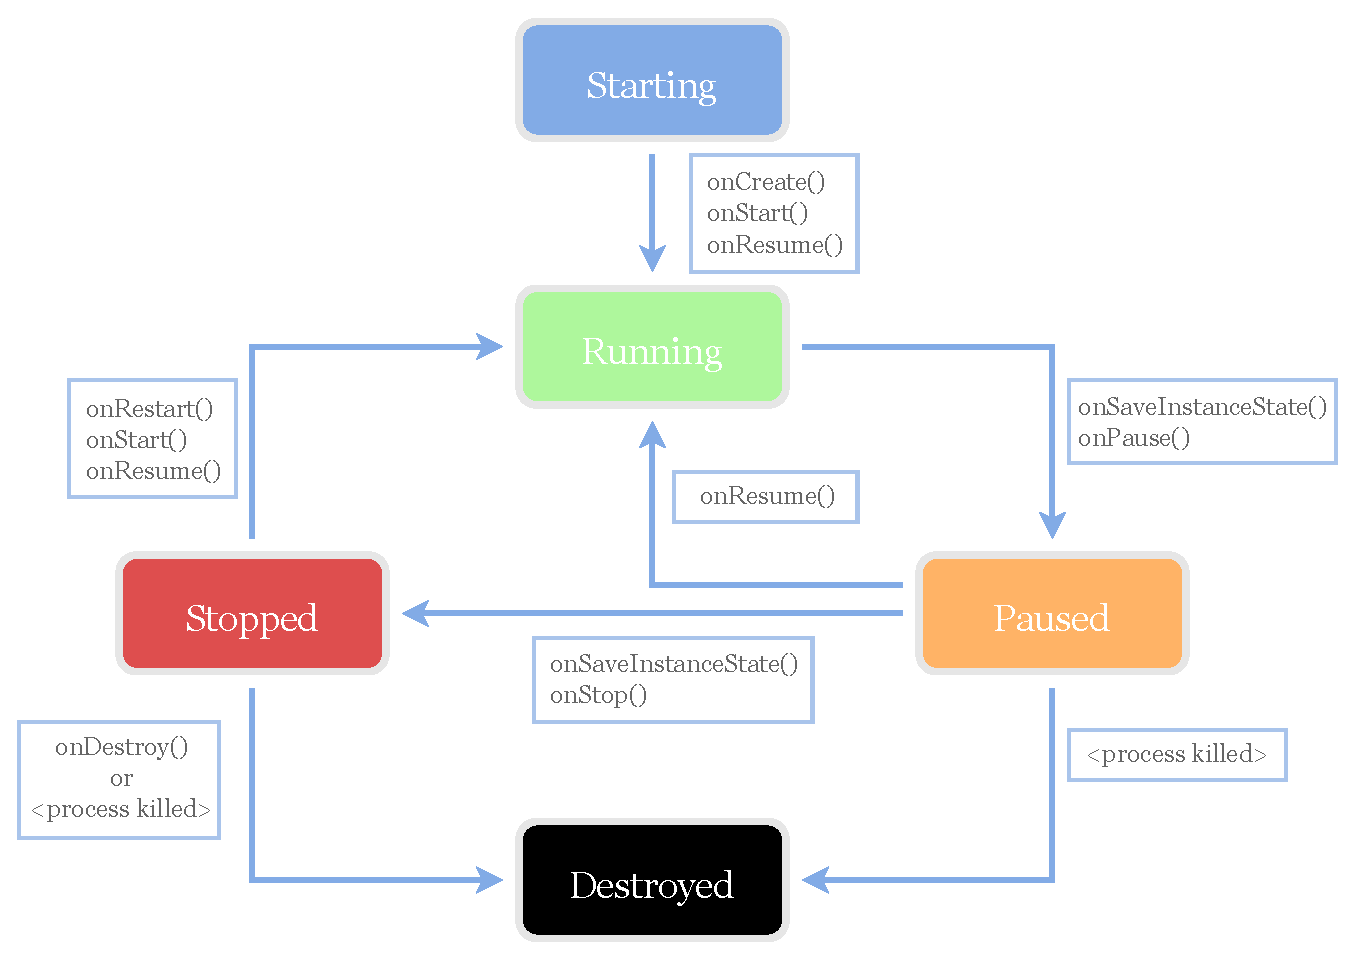
\includegraphics[scale=0.7]{android_lifecycle.eps}
                \caption*{Ciclo de vida de actividades Android}
                \label{fig:androidlifecycle}
        \end{figure}

\section{Pruebas llevadas a cabo}

% describiranse as probas realizadas aos distintos niveis para

% garantir o correcto funcionamento do software ou do hardware.

\section{Manual de usuario}
    \subsection{Requisitos mínimos}
        Para poder utilizar el sistema \textbf{Wifither} se debe cumplir un conjunto de requisitos, los cuales están especificados a continuación.

        \begin{itemize}
            \item Equipo con una distrubución GNU/Linux para compilar paquete. Ubuntu como subsistema de Windows, BSD o MacOS no están oficialmente soportados, aunque suelen dar buenos resultados. Cygwin no está soportado debido al sistema de archivos que utiliza, que no es capaz de distinguir entre mayúsculas y minúsculas.
            \item Router con sistema operativo OpenWRT donde se ejecutará el servicio servidor.
            \item Dispositivo móvil con sistema operativo Android donde se instalará la aplicación cliente.
            \item Conexión a Internet tanto en el router como en el dispositivo móvil.
        \end{itemize}

        \todo{redactar mejor}
        Aunque muchas de las dependencias necesarias suelen venir por defecto instaladas en diferentes sistemas operativos, es necesario que todas estén instaladas y funcionales. A continuación se muestra una tabla con las dependencias y el nombre de los paquetes en distribuciones \textit{Debian-like} \todo{modificar dependiendo de la tabla}

        \todo{debería poner toda la tabla? o quitar arch? o quitar todo?}
        %\begin{table}
            \begin{tabular}{|l|l|l|}
                \hline
                \textbf{Prerequisitos}  & \textbf{Debian}   & \textbf{Arch}             \\           
                \hline
                asciidoc                & asciidoc          & asciidoc                  \\
                GNU Bash                & bash              & bash                      \\
                GNU bc                  & bc                & bc                        \\
                GNU Binutils            & binutils          & binutils                  \\
                bzip2                   & bzip2             & bzip2                     \\
                fastjar                 & fastjar           & fastjar                   \\
                flex                    & flex              & flex                      \\
                git                     & git-core          & git                       \\
                GNU C++ Compiler        & g gcc-c           & -                         \\
                GNU C Compiler          & gcc               & gcc                       \\
                getopt                  & util-linux        & util-linux                \\
                GNU awk                 & gawk              & gawk                      \\
                gtk2.0-dev              & libgtk2.0-dev     & gtk2                      \\
                intltool-update         & intltool          & intltool                  \\
                jikes                   & jikespg           & -                         \\
                libz, libz-dev          & zlib1g-dev        & zlib                      \\
                Mercurial / hg          &                   & mercurial                 \\
                make                    & make              & make                      \\
                mkisofs                 & genisoimage       & cdrkit                    \\
                ncurses                 & libncurses5-dev   & ncurses                   \\
                openssl/ssl.h           & libssl-dev        & openssl                   \\
                patch                   & patch             & patch                     \\
                perl-ExtUtils-MakeMaker & perl-modules      & perl-extutils-makemaker   \\
                python2.6-dev           & python2.6-dev     & python2                   \\
                rsync                   & rsync             & rsync                     \\
                ruby                    & ruby              & ruby                      \\
                sdcc                    & sdcc              & sdcc                      \\
                subversion              & subversion        & subversion                \\
                unzip                   & unzip             & unzip                     \\
                GNU Wget                & wget              & wget                      \\
                xgettext                & gettext           & gettext                   \\
                xsltproc                & xsltproc          & libxslt                   \\
                zlib, zlib-static       & zlib1g-dev        & zlib                      \\
                \hline
            \end{tabular}
        %\end{table}

        Para instalar paquetes en distribuciones \textit{Debian-like} su utiliza el siguiente comando.
        Es necesario que el usuario desde el que se ejecute el comando de instalación cuente con los permisos necesarios para llevar a cabo dicha acción.

        \todo{Estilos de estos códigos}
        \begin{lstlisting}[language=bash]
            $ apt-get install <paquete>
        \end{lstlisting}

        Varios paquetes pueden ser instalados a la vez utilizando el comando solo una vez.
        Ejemplo:

        \begin{lstlisting}[language=bash]
            $ apt-get install libncurses5-dev subversion gawk
        \end{lstlisting}

    \subsection{Manual de instalación}
    
        
        \subsubsection{Compilar el paquete Wifither para OpenWRT}
            Para preparar la compilación cruzada, descargar desde la página web oficial de OpenWRT \url{https://downloads.openwrt.org} el SDK correspondiente al modelo del dispositivo y la versión del sistema en el que se desea instalar el paquete. Una vez descargado, descomprimir el archivo y se copiar el código fuente dentro de la carpeta \textit{build} del SDK. Luego, desde la carpeta raíz del SDK, ejecutar los siguientes comandos para preparar las librerías que utiliza \textbf{Wifither}.

            \begin{lstlisting}[language=bash]
                $ ./scripts/feeds update
                $ ./scripts/feeds install uclibcxx
                $ ./scripts/feeds install libopenssl
            \end{lstlisting}

            Una vez esté todo preparado, ejecutar el comando \textit{make} para llevar a cabo la compilación. El paquete resultante se almacena en \textit{SDK/bin/<modelo-router>/packages/base} con el nombre \textit{wifither 1 <modelo-router>.ipk}.


        \subsubsection{Instalación del servicio servidor en e router}
            En este apartado se explica cómo instalar el paquete \textit{.ipk} resultante de la compilación, en el router con OpwenWRT, cómo arrancar iniciar el servicio y configurarlo para que inicie automáticamente cada vez que inicie el router.

            Primeramente se debe copiar el paquete al router donde se instalará, para ello se puede utilizar cualquier protocolo de red que permita la transferencia de archivos, en esta guía se explica cómo copiarlo mediante el uso de \textit{scp}. Para realizar este proceso, se debe especificar la ruta donde se encuetra el paquete, el usuario y equipo remoto al que se desea copiar, y la ruta donde se desea almacenar en ese equipo.

            \begin{lstlisting}[language=bash]
                $ scp <ruta-paquete> <usuario>@<equipo-remoto>:<ruta-almacenamiento>
            \end{lstlisting}

            Un ejemplo de la ejecución del comando:
            \begin{lstlisting}[language=bash]
                $ scp bin/brcm63xx/packages/base/wifither_1_brcm63xx.ipk root@192.168.0.4:/root/wifither
            \end{lstlisting}

            Una vez el paquete está en el router, este podrá ser instalado utilizando el gestor de paquetes de OpenWRT \textit{opkg}
            \begin{lstlisting}[language=bash]
                $ opkg install <ruta-paquete>
            \end{lstlisting}

            Para iniciar el servicio después de haberlo instalado se ejecutará \textit{wifiter} especificando el puerto en el que se desea recibir los paquetes y una contraseña que contenga al menos ocho caracteres.

            Ejemplo:
            \begin{lstlisting}[language=bash]
                $ wifither 4848 Potato12
            \end{lstlisting}

            Para configurar el equipo, de forma que Wifither siempre se inicie al arrancar el sistema, se debe editar el archivo \textit{/etc/rc.local} añadiendo la ejecución del servicio antes de la línea \textit{exit 0}

            \begin{lstlisting}[language=bash]
                # Put your custom commands here that should be executed once
                # the system init finished. By default this file does nothing.

                wifither 4848 Potato12

                exit 0
            \end{lstlisting}


        \subsubsection{Instalación de la aplicación móvil}
            Para realizar la instalación de la aplicación en el móvil existen dos opciones, utilizar la aplicación ya compilada \textit{.apk} o compilarla e instalarla directamente desde \textit{Android Studio}
            
            \begin{enumerate}
                \item Instalación del .apk
                Es necesario que el archivo \textit{.apk} debe estar almacenado en el dispositivo móvil, para esto se puede conectar el dispositivo directamente al ordenador utilizando un cable USB.

                Para llevar a cabo la instalación debe estar activada la opción \textit{Fuentes desconocidas}, que se encuentra en el apartado \textit{Seguridad} de los ajustes del sistema Android. Esto hace que sea posible la instalación de aplicaciones que provengan de fuentes no oficiales.

                Una vez realizados los pasos anteriores, ir hasta la ubicación del archivo \textit{.apk}, pulsar sobre él y aceptar la instalación.

                \item Compilar e instalar desde Android Studio
                Para poder instalar aplicaciones utilizando este método es necesario que el dispositivo móvil esté conectado al ordenador mediante un cable USB y que esté activada la opción \textit{Depuración USB}, que se encuentra en el apartado \textit{Opciones de desarrollador} de los ajuste del sistema Android.
                \textbf{NOTA:} Las opciones de desarrollador están deshabilitadas por defecto en la mayoría de dispositivos Android, para habilitarla es necesario pulsar diez (10) veces sobre el \textit{Número de compilación}, que se encuentra en el apartado \textit{Acerca del dispositivo} de los ajuste del sistema Android.

                En la barra de menús de Android Studio, ir a \textit{File} y luego a la opción \textit{Open}, allí buscar y abrir la carpeta con el código fuente de la aplicación. Una vez haya cargado el proyecto, ir la opción \textit{Run `app'} que se encuentra en el menú \textit{Run} y seleccionar el dispositivo.
                
                \textbf{NOTA:} Es importante aceptar en el dispositivo la clave RSA, esto permite que Android Studio pueda conectarse al dispositivo.

                Tras realizar los pasos anteriores, el código fuente debe haber quedado compilado, instalado y ejecutado en el dispositivo conectado.
            \end{enumerate}

        \todo{ddns, segundo router o router principal?}

        \subsubsection{Configuración de una VPN} \todo{cómo poner opcional?}
            En este apartado se explica la creación y configuración de una VPN en modo tunel entre el router y el dispositivo móvil mediante la utilización de OpenVPN. Esto paso es totalmente opcional ya que el sistema no lo necesita para su correcto funcionamiento, sin embargo, añade una capa de seguridad adicional que permite que todo el tráfico entre cliente y servido sea encriptado en origen y desencriptado en destino, por lo que nunca se conoce el contenido real de los paquetes enviados y no pueden ser replicados.

            \begin{enumerate}
                \item Creación de VPN en el router \todo{Añadir un enter y revisar el resto}
                    Inicialmente se debe comprobar que los repositorios desde los que descargan los paquetes y librerías estén bien configurados en el router. Esto se puede observar en el archivo de configutación \textit{/etc/opkg/dist-feeds.conf}. Las rutas a los diferentes repocitorios dependerán de la versión del sistema y el modelo del router.

                    Ejemplo:
                    \url{https://downloads.openwrt.org}

                    \begin{lstlisting}[language=bash]
                        src/gz designated_driver http://downloads.openwrt.org/snapshots/trunk/brcm63xx/smp/packages/packages
                        src/gz designated_base http://downloads.openwrt.org/snapshots/trunk/brcm63xx/smp/packages/base
                        src/gz designated_packages http://downloads.openwrt.org/snapshots/trunk/brcm63xx/smp/packages/packages
                        src/gz designated_luci http://downloads.openwrt.org/snapshots/trunk/brcm63xx/smp/packages/luci
                        src/gz designated_routing http://downloads.openwrt.org/snapshots/trunk/brcm63xx/smp/packages/routing
                        src/gz designated_telephony http://downloads.openwrt.org/snapshots/trunk/brcm63xx/smp/packages/telephony
                        src/gz designated_management http://downloads.openwrt.org/snapshots/trunk/brcm63xx/smp/packages/management
                    \end{lstlisting}
                    
                    Con los repositorios bien configurados, instalar \textit{openvpn-openssl} y \textit{openvpn-easy-rsa}
                    
                    \begin{lstlisting}[language=bash]
                        $ opkg update
                        $ opkg install openvpn-openssl openvpn-easy-rsa
                    \end{lstlisting}

                    \todo{Cómo funciona esto? Privado público?}
                    A continuación se deben crear los certificados de seguridad para cliente y servidor. El siguiente código crea un certificado servidor con el nombre \textit{my-server} y un ccertificado cliente con el nombre \textit{my-client}. Se peuden crear tantos certificados clientes como sean necesarios ejecutando el mismo comando de creación \textit{build-key-pkcs12} varias veces especificando diferentes nombres.

                    \begin{lstlisting}[language=bash]
                        $ build-ca
                        $ build-dh
                        $ build-key-server <nombre-clave-servidor>
                        $ build-key-pkcs12 <nombre-clave-cliente>
                    \end{lstlisting}

                    Una vez generadas las claves:
                    
                        \begin{itemize}

                            \item Copiar las perteneciantes al servidor servidor en el directorio \textit{/etc/openvpn}
                            \begin{lstlisting}[language=bash]
                                $ cp /etc/easy-rsa/keys/ca.crt /etc/easy-rsa/keys/clave-servidor.* /etc/easy-rsa/keys/dh2048.pem /etc/openvpn
                            \end{lstlisting}

                            \item Copiar las pertenecientes al cliente en el dispositivo móvil mediante cualquier método disponible, puede ser a través de un dispositivo USB, un eMail, scp, etc.
                            Ejemplo: Copiar las claves al equipo desde el que se compiló el paquete y conectar allí el dispositivo móvil
                            \begin{lstlisting}[language=bash]
                                $ scp /etc/easy-rsa/keys/ca.crt /etc/easy-rsa/keys/clave-cliente.* root@192.168.0.100:/etc/openvpn
                            \end{lstlisting}
                        \end{itemize}   
                    
                    A continuación se muestran los comandos a ejecutar para la creación y configuración de una nueva red en el router por la que se realizarán las conexiones de la VPN y la configuración del cortafuegos correspondiente.

                    \begin{enumerate}
                        \item Crear la nueva interfaz de la VPN con el nombre vpn0
                            
                        \begin{lstlisting}[language=bash]
                            $ uci set network.vpn0=interface
                            $ uci set network.vpn0.ifname=tun0
                            $ uci set network.vpn0.proto=none
                            $ uci set network.vpn0.auto=1        
                        \end{lstlisting}

                        \item Configurar el cortafuegos para permitir conexiones entrantes al puerto \textit{1194} (puerto por defecto).

                        \begin{lstlisting}[language=bash]
                            $ uci set firewall.Allow_OpenVPN_Inbound=rule
                            $ uci set firewall.Allow_OpenVPN_Inbound.target=ACCEPT
                            $ uci set firewall.Allow_OpenVPN_Inbound.src=*
                            $ uci set firewall.Allow_OpenVPN_Inbound.proto=udp
                            $ uci set firewall.Allow_OpenVPN_Inbound.dest_port=1194    
                        \end{lstlisting}

                        \item Crear nueva zona nombrada \textit{vpn} para la red vpn0. Esto permitirá las conexiones relacionadas con el tunel VPN, tanto entrantes como salientes.

                        \begin{lstlisting}[language=bash]
                            $ uci set firewall.vpn=zone
                            $ uci set firewall.vpn.name=vpn
                            $ uci set firewall.vpn.network=vpn0
                            $ uci set firewall.vpn.input=ACCEPT
                            $ uci set firewall.vpn.forward=REJECT
                            $ uci set firewall.vpn.output=ACCEPT
                            $ uci set firewall.vpn.masq=1
                        \end{lstlisting}

                        \item Aplicar la nueva configuración.

                        \begin{lstlisting}[language=bash]
                            $ uci commit network
                            $ /etc/init.d/network reload
                            $ uci commit firewall
                            $ /etc/init.d/firewall reload  
                        \end{lstlisting}

                        \item Configuración de OpenVPN:
                        La configuración puede ser realizada medainte los archivos \textit{.conf} de OpenVPN o a través de la interfaz \textit{uci} de OpenWRT. En esta guía se indican los comandos a ejecutar para realizarlo mediante esta última opción.

                        \begin{lstlisting}[language=bash]
                            $ echo > /etc/config/openvpn
                            $ uci set openvpn.myvpn=openvpn
                            $ uci set openvpn.myvpn.enabled=1
                            $ uci set openvpn.myvpn.verb=3
                            $ uci set openvpn.myvpn.port=1194
                            $ uci set openvpn.myvpn.proto=udp
                            $ uci set openvpn.myvpn.dev=tun
                            $ uci set openvpn.myvpn.server='10.8.0.0 255.255.255.0'
                            $ uci set openvpn.myvpn.keepalive='10 120'
                            $ uci set openvpn.myvpn.ca=/etc/openvpn/ca.crt
                            $ uci set openvpn.myvpn.cert=/etc/openvpn/my-server.crt
                            $ uci set openvpn.myvpn.key=/etc/openvpn/my-server.key
                            $ uci set openvpn.myvpn.dh=/etc/openvpn/dh2048.pem
                            $ uci commit openvpn
                        \end{lstlisting}

                        \item Iniciar OpenVPN
                        \begin{lstlisting}[language=bash]
                            $ /etc/init.d/openvpn enable
                            $ /etc/init.d/openvpn start
                        \end{lstlisting}
                    \end{enumerate}

                \item Conexión al la VPN desde dispositivo Android
                Para establecer la conexión con la VPN se debe instalar la aplicación \textit{OpenVPN for Android} desde \textit{Google Play Store}
                
                \url{https://play.google.com/store/apps/details?id=de.blinkt.openvpn}

                Una vez instalada la aplicación, añadir un nuevo perfil desde la pestaña \textit{Profiles} presionando el botón \textit{Add Profile} y especificando un nombre. Después de realizar el paso anterior, en la pestaña \textit{Basic}, seleccionar \textit{PKCS12 File} como el tipo de autenticación a utilizar, luego presionar el botón \textit{Select...} de la parte superior y buscar en el almacenamiento el archivo copiado al dispositivo en el apartado anterior \textit{<nombre-clave-cliente>.p12}. Opcionalmente se puede añadir la contraseña en el apartado \textit{Password} para que se introduzca autmáticamente al iniciar sesión.

                Finalmente entrar en la pestaña \textit{Server List} y especificar la dirección del servidor OpenWRT en el apartado \textit{Server Address}, y en el apartado \textit{Server Port} especificar el puerto configurado en el servidor (1194 por defecto).

                Después de haber configurado la aplicación, se puede establecer conección con la VPN presionando sobre el perfil creado. A partir de estre punto, todas las conexiones entre cliente y servidor serán cifradas.
            \end{enumerate}

    \subsection{Manual de utilización}
        \todo{references??????}
        En esta sección se explican las funcionalidades que tiene la aplicación y cómo utilizarlas, en las imágenes \ref{fig:main_activity_manual} y \ref{fig:devices_activity_manual} se encuentran enumerados los elementos de la interfaz que son explicados a continuación.

        \begin{figure}[h!]
            \centering
                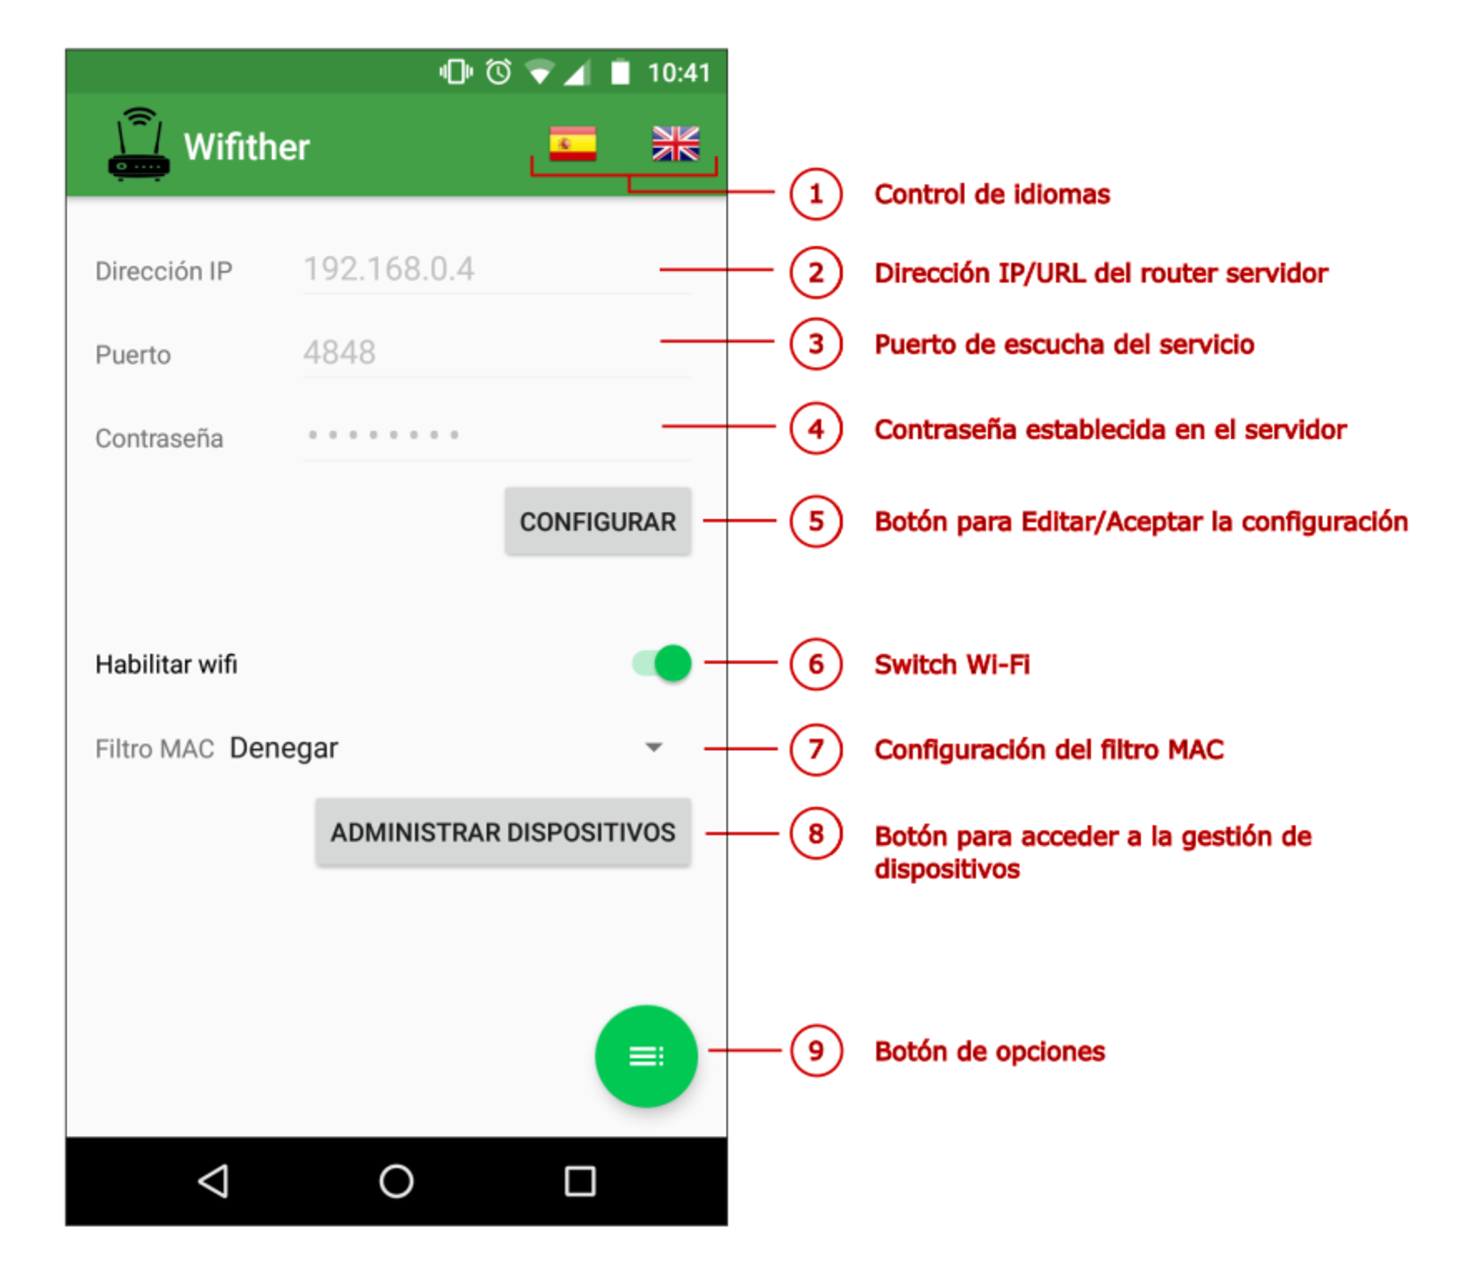
\includegraphics[scale=0.5]{main_activity_manual.eps}
                \caption*{Vista principal}
                \label{fig:main_activity_manual}
        \end{figure}

        \todo{Y la organización de esto???}
        \begin{figure}[h!]
            \centering
                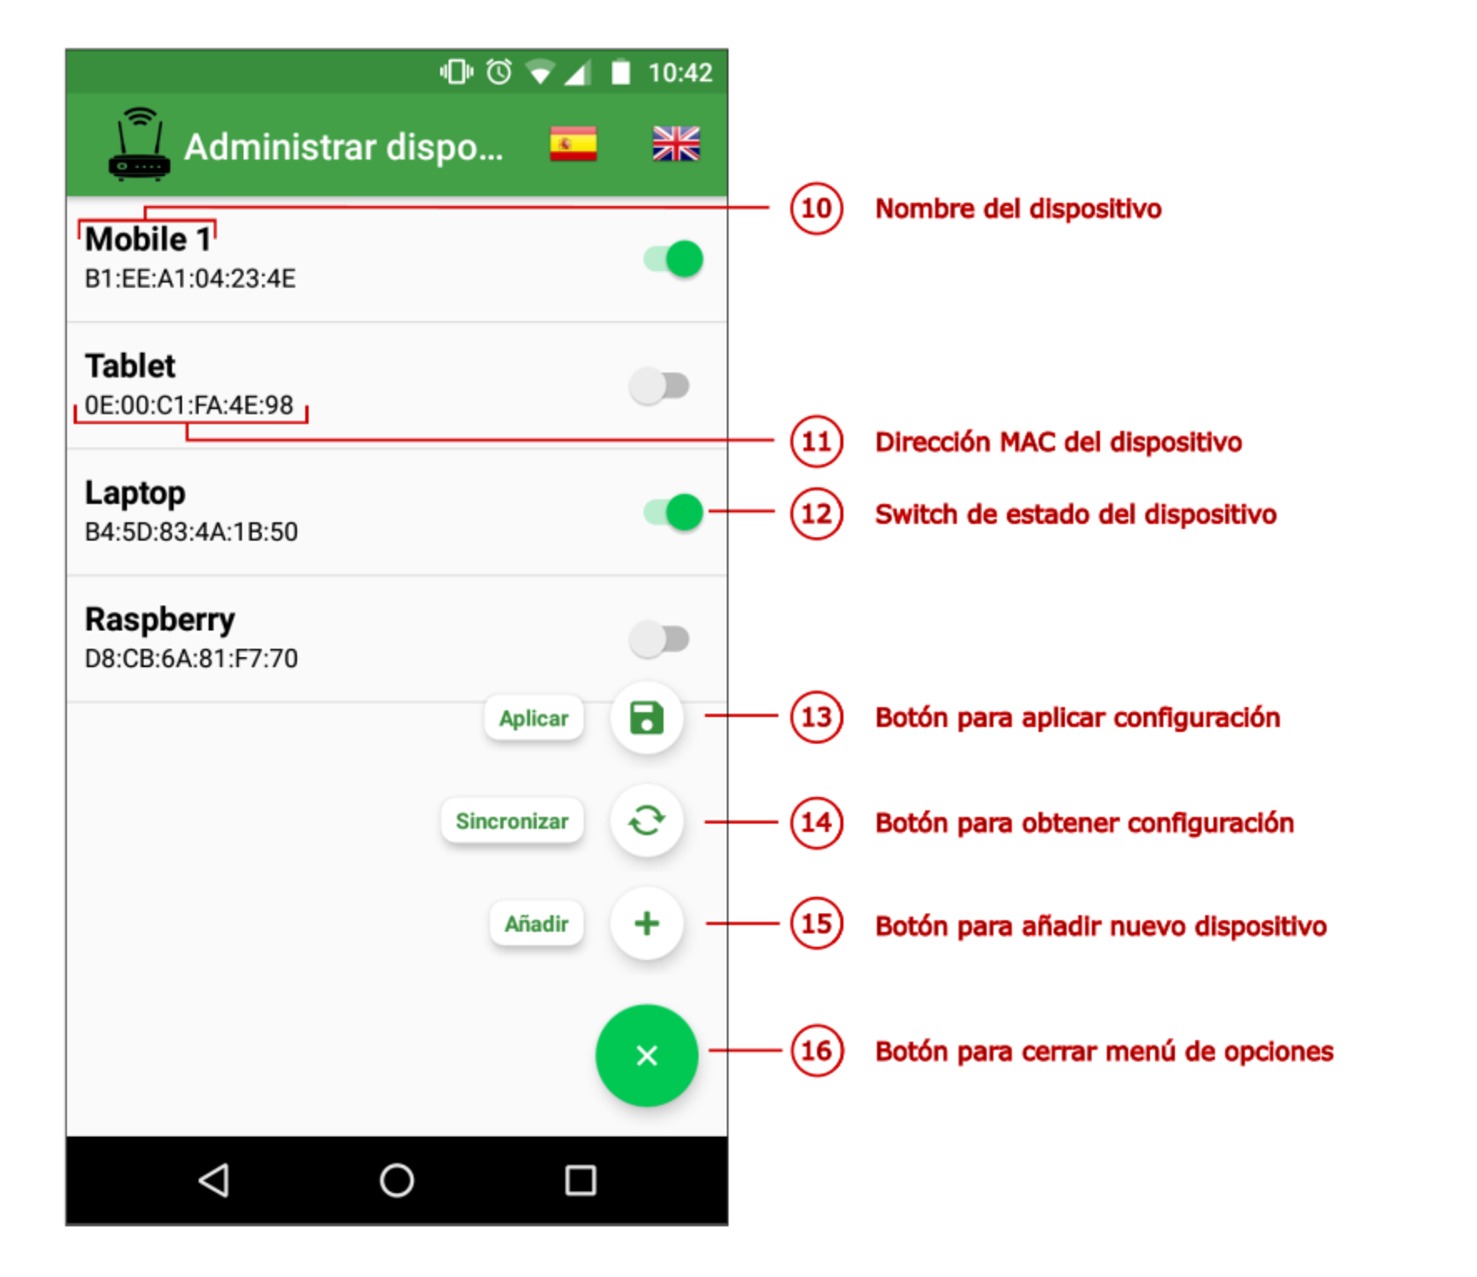
\includegraphics[scale=0.5]{devices_activity_manual.eps}
                \caption*{Administración de dispositivos}
                \label{fig:devices_activity_manual}
        \end{figure}

        \begin{enumerate}

            \item Control de idiomas
            Permite seleccionar el idioma con el que se muestran las opciones de la interfaz de usuario, están disponibles castellano e inglés, el idioma por defecto de la aplicación es el inglés.

            \item Dirección IP/URL del rputer servidor
            Es el campo de texto donde se especifica la dirección del router OpenWRT en el cual se ha instalado la aplicación y sobre el que se desea gestionar la red Wi-Fi. La edición de este campo está deshabilitada por defecto, para cambiar su contenido se debe hacer uso del botón señalado con el número 5 en la \ref{fig:main_activity_manual}

            \item Puerto de escucha del servicio
            Es el puerto que se indica al iniciar la aplicación en el router OpenWRT y que se utiliza para recibir las órdenes desde el dispositivo móvil. La edición de este campo está deshabilitada por defecto, para cambiar su contenido se debe hacer uso del botón señalado con el número 5 en la \ref{fig:main_activity_manual}

            \item Contraseña establecida en el servidor
            Es la contraseña que se indica al iniciar la aplicación en el router OpenWRT y que se utiliza para encriptar y desencriptar las órdenes enviadas desde el dispositivo móvil. La contraseña debe contener al menos ocho caracteres. La edición de este campo está deshabilitada por defecto, para cambiar su contenido se debe hacer uso del botón señalado con el número 5 en la \ref{fig:main_activity_manual}

            \item Botón para Editar/Aceptar la configuración
            Este botón habilita la edición de los campos de configuración señalados con los números 1, 2 y 3 en la \ref{fig:main_activity_manual}. Tras ser pulsado, el texto del botón cambia a \textit{Confirmar}, y debe ser pulsado para guardar la nueva configuración.

            \item Switch Wi-Fi
            Enciende o apaga la red Wi-Fi en el router OpenWRT, la posición iquierda indica que la red Wi-Fi está apagada, la posición hacia la derecha indica que está encendida.

            \item Configuración del filtro MAC
            Permite seleccionar la configuración del filtro MAC en el router OpenWRT. El selector tiene tres posiciones: \textit{Deshabilitado}, \textit{Permitir} y \textit{Denegar}.
            \begin{itemize}
                \item Si el filtro MAC está deshabilitado, cualquier dispositivo puede conectarse a la red Wi-Fi sin restricción de ningún tipo.
                \item Si el filtro MAC está configurado para \textit{Permitir}, significa que sólo pueden acceder a la red Wi-Fi los dispositivos que hayan sido especificados para que el filtro les sea aplicado.
                \item Si el filtro MAC está configurado para \textit{Denegar}, significa que tienen acceso a la red todos los dispositivos excepto los especificados para que el filtro les sea aplicado.
            \end{itemize}
            
            \item Botón para acceder a la gestión de dispositivos
            Al pulsarlo se accede a un nuevo conjunto de opciones desde donde se pueden adicionar, editar y eliminar dispositivos, además de poder seleccionar los dispositivos con los que se desea aplicar el filtro MAC.
            \item Botón de opciones
            Permite acceder a las opciones marcadas con los puntos 12, 14 y 15 en la \ref{fig:devices_activity_manual}
            \item Nombre del dispositivo
            Es un indicador distintivo para cada dispositivo, es determinado por el usuario al añadir un nuevo dispositivo y es un campo obligatorio.
            \item Dirección MAC del dispositivo
            Identificador único del adaptador de red del dispositivo. Es especificado por el usuario al añadir un nuevo dispositivo y debe cumplir con un formato específico compuesto por seis pares de caracteres hexadecimales separados por dos puntos(:). Si el formato introducido no es correcto, el botón \textit{Añadir} queda deshabilitado.
            \item Switch de estado del dispositivo
            Añade o elimina dispositivos para que se le aplique la configuración del filtro MAC, la posición iquierda indica que la configuración del filtro \textbf{NO} se aplica al dispositivo, la posición hacia la derecha indica que la configuración del filtro \textbf{NO} se aplica al dispositivo.
            \item Botón para aplicar configuración
            Aplica en el router OpenWRT la configuración que haya sido establecida.
            \item Botón para optener configuración.
            Actualiza el dispositivo móvil con la configuración actual del router OpenWRT. Esta opción es útil cuando se gestiona la red desde más de un dispositivo móvil, de esta forma cada dispositivo puede saber siempre la última configuración aplicada en el router.
            \item Botón para añadir nuevo dispositivo
            Muestra un cuadro de diálogo que permite introducir los datos del nuevo dispositivo y añadirlo a la lista de dispositivos
            \item Botón para cerrar el menú de opciones
            Cierra el menú de opciones, también puede ser cerrado presionando sobre cualquier espacio fuera del menú.
            
        \end{enumerate}

        \todo{subsection??}
        Para editar la información de un dispositivo, mantener pulsado sobre el mismo hasta que aparezca un cuadro de diálogo y seleccionar la opción editar. La información del dispositivo debe cumplir los siguientes requisitos: El nombre de dispositivo no puede estar vacío, y la dirección MAC debe estar compuesta por seis pares de caracteres hexadecimales separados por dos puntos(:)

        Para editar la información de un dispositivo, mantener pulsado sobre el mismo hasta que aparezca un cuadro de diálogo y seleccionar la opción eliminar.

        \textbf{IMPORTANTE:} Debe tenerse en cuenta que una mala configuración del filtro MAC puede provocar la pérdida de la conexión en el dispositivo desde el que se está gestionando la red Wi-Fi si está directamente conectado a esta. La configración establecida debe ser revisada cautelosamente antes de ser aplicada. En caso de pérdida de conexión por este motivo, contactar con el encargado/a de instalar y configrar la aplicación en el router OpenWRT.

\section{Conclusiones y trabajo futuro}


    \subsection{Principales aportaciones}

    % deberanse destacar entre 3 e 5 aportacións importantes do

    % traballo realizado, tendo en conta os obxectivos fixados.


    \subsection{Conclusiones}

    % incluiranse todas as conclusións de tipo técnico e persoal.


    \subsection{Trabajo futuro}
    % presentaranse posible ampliacións e traballos relacionados por facer.


\section{Referencias}
``I always thought something was fundamentally wrong with the universe'' \citep{adams1995hitchhiker}
https://www.internetworldstats.com/stats.htm \citep{hola}
% deberanse citar todas as fontes de información empregadas para a realización do traballo.

% 1. Autor/a/es/as.

% 2. Título do artigo, libro, monografía,...

% 3. Editorial ou nome da revista.

% 4. Número da revista, volume e páxinas (só para revistas).

% 5. Ano de publicación.

% 6. Dirección e data de consulta (só para URL).

% Recoméndase empregar para referencias de artigos, revistas, e outras fontes de

% referencia, o formato APA, ISO 690, IEEE ou similares, e uniformizados ao longo de

% toda a sección.

% Deberase empregar un estilo uniforme para todas elas e aportarase, en cada caso:

\section{Anexos}

% incluiranse outros elementos de interese no TFG que se consideren necesarios para a

% mellor comprensión do mesmo.

\section{Tecnologías}
\todo{debería empezar por ``Es tal cosa'' siempre o meejor empezar con el nombre, o sin nada?}
    \subsection{OpenWRT}
        OpenWRT es una distribución Linux para dispositivos embebidos\todo{y routers}. En lugar de existir como un firmware estático, OpenWRT proporciona un sistema de archivos totalente modificable con gestión de paquetes, el cuál permite sustituir el sistema del proveedor y una mayor personalización del dispsitvo. Es el framework perfecto para el desarrollo de una aplicación sin tener que construir todo el firmware que a rodee.

    \subsection{C}
        Es un lenguaje de programación imperativo de prósito general que destaca por la eficiencia de su código y su popularidad para crear software de sistemas debido a su flexibiliadad y control a muy bajo nivel. Es la opción ideal cuando se desea ahorrar la mayor cantidad de espacio posible en la construcción del software, necesidad común de dispositivos embebidos. \todo{solo embebidos?}

        \subsubsection{OpenWRT SDK}
            El SDK es un conjunto de herramientas de programación reubicables y precompiladas que permiten la compilación cruzada de paquetes para el espacio de usuario de OpenWRT\todo{ref openwrt} sin tener que compilar todo el sistema desde cero.

        \subsubsection{uClibc}
            \todo{yewClibc}
            Es una librería \todo{en?}C para el desarrollo de sistemas Linux embebidos, es más pequeña que la librería \todo{poner estilo} glibc (GNU C Library) y soporta prácticamente todas las aplicaciones que son desarrolladas con esta. uClibc \todo{yewClibc} es capaz de gestionar librerías compartidas e hilos, además de funcionar con procesadores de varias arquitectura, entre las que se incluyen amd64, ARM, mips/mipsel, alpha, PowerPC y SH.

        \subsubsection{OpenSSL}
            Es un proyecto de código abierto que implementa la una librería criptográfica de propósito general. Provee un conjuto de herramientas robusto, de nivel comercial, para los protocolos SSL/TLS.

    \subsection{OpenVPN}
        \todo{openvpn}

    \subsection{sed}
        Es una utilidad unix, un editor de flujo capaz de analizar y transformar textos utilizando un simple y compacto lenguaje de programación. Permite el uso de expresiones regulares y tratamiento de archivos con un gran número de líneas de forma rápida.

    \subsection{\LaTeX}\todo{debería ir así?}
        Es un sistema de tipografía de alta calidad, incluye mecanismos diseñados para la creación de documentación científica y técnica por lo que se ha convertido en el estándar de facto a la hora de desarrollar esta tarea. Está concebido como siftware libre, y cuenta con múltiples librerías que añaden funcionalidades comunmente necesarias para la creación de estos doumentos.

    \subsection{Java}
        Es un lenguaje de programación orientado a objetos, compilado, de propósito general y alto nivel. Es el principal lenguaje para el desarrollo de aplicaciones móviles Android, además de ser utilizado para soluciones web, cliente-servidor, sistemas distribuidos, etc.

    \subsection{Git}
        Es un sistema de control versiones distribuido diseñado para controlar proyectos de cualquier tamaño con rapidez y eficacia. Es de código abierto y ofrece medios para guardar, analizar y revertir cambios realizados en versiones actuales y anteriores, además del control de ramas que permite mantener y trabajar en más de una versión de un proyecto de forma simultánea.

\section{Herramientas} \todo{Herraminetas?}
    \todo{justificación de la utilización? no llega con explicar las caracterísiticas que lo distinguen?}
    \subsection{Atom}
        Es un editor de texto de código abierto desarrollado por GitHub Inc.,\todo{Qué hago aquí?} escrito en JavaScript, moderno, accesible y modificable en su totalidad. Es completamente personalizable, de forma que brinda el entorno de trabajo más cómodo y productivo posible, sin necesidad de modificar ningún archivo de configuración durante el desarrollo de proyectos. Cuenta con una muy amplia gama de paquetes, también de código abierto, que añaden y mejoran funcionalidades del editor.

    \subsection{Visual Studio Code}
        Es una herramienta desarrollada por Microsoft que combina las simplicidad de un editor de texto con lo que necesitan los desarrolladores para su ciclo básico ``edit-build-debug'' \todo{style}. Visual Studio Code provee soporte exhaustivo para la creación y depuración de código, además de un modelo extendible y una integración de bajo consumo de recursos con las herramientas existentes.

    \subsection{TeX Live}
        Es un una distribución libre para los sistemas de tipografía TeX\todo{ref latex}. Está disponible para Linux y Windows incluyendo la mayoría de programas, micro paquetes y fuentes que son software libre. Actualmente es la distribución por defecto de esta tecnología en múltiples distribuciones Linux como openSUSE, Fedora, Debian, Ubuntu y Gentoo, además de ofrecer soporte para múltiples idiomas.

    \subsection{Android Studio}
        Es el \todo{estilo}IDE (Integrated development environment) oficial para la creación aplicaciones Android. Ofrece herramientas para la edición de códigos de primer nivel, depuración, control de rendimiento y compilación instantánea. \todo{releer}Provee de un emulador Android que permite comprobar el funcionamiento del código de forma rápida y brinda un conjunto de opciones dinámicamente configurables en cuanto a tamaño, prestaciones y control de sensores. Posee integración condiferentes sitemas actuales y cuenta con soporte para librerías externas configurables para su compilación junto con la aplicación.

    \subsection{GitHub}
        Es una plataforma colaborativa de control de vesiones online basada en Git\todo{ref git} y desarrollada por GitHub Inc. Ofrece todas las funcionalidades de gestión de códigos que ofrece Git\todo{ref git} así como sus propias características basadas en la web. Provee control de acceso y varias opciones colaborativas como el control de errores, petición de funcionalidades, gestión de tareas y wikis. La plataforma cuenta con un servicio de pago que permite la creación de repositorios privados, este servicio está disponible de forma gratuita junto a un conjunto de herramientas de desarrollo que la empresa ofrece en un paquete para estudiantes verificados.

    \subsection{Lucidchart}
        Es una aplicación online enfocada a la creación de diagramas profesionales desde una interfaz web. Es una herramienta realmente cómoda a la hora de documentar proyectos grandes debido a lo sencillo y amigable de su entorno. Además, brinda integración con diferentes aplicaciones externas como Dropbox, Slack y Microsoft Office. 

    \subsection{Inkscape}
        Es un editor profesional de gráficos vectoriales disponible para Windows, Mac OS X y Linux. Es de código abierto y soporta una gran variedad de formatos, entre los que se incluye \textit{.eps}, el formato utilizado por latex. Además brinda una amplia variedad de herramientas para realizar trazado vectorial, manipulación de objetos y edición de textos.
        \todo{revisar}

    \subsection{OpenVPN for Andorid}
    \todo{hacer}

\bibliographystyle{plain}
\bibliography{references}

\end{document}
